Consider following unity gain feedback system. 
\begin{center}
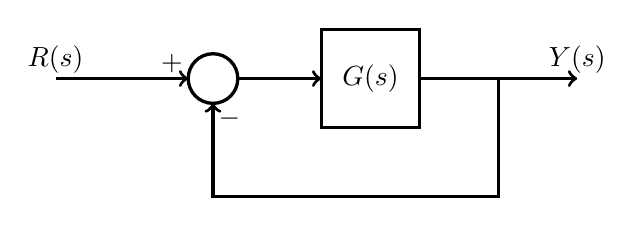
\begin{tikzpicture}[scale=1,inner sep=0pt,outer sep=0pt,very thick,
sysblock/.style={draw,rectangle,inner sep=2pt,minimum width=1.25cm,minimum height=1.25cm,inner sep=4pt, very thick}]
\draw (2,0) node[draw,circle] (sum1) {$\rule{0pt}{18pt}$};
%\draw (4,0) node[sysblock] (K) {$K$};
\draw (4,0) node[sysblock] (G) {$G(s)$};
\draw[->] (0,0) node[above=2pt] {$R(s)$} -- (sum1.180) node[above left=2pt] {$+$};
%\draw[->] (sum1.0)  -- (K.180);
%\draw[->] (K.0) -- (G.180);
\draw[->] (sum1.0) -- (G.180);
\draw[->] (G.0) -- ++(2,0) node[above=2pt] {$Y(s)$};
\draw[->] (G.0) ++(1,0) -- ++(0,-1.5) -| (sum1.-90) node[below right=2pt] {$-$};
\end{tikzpicture}
\end{center}
The Bode plot of $G(s)$ is shown below. $G(s)$ is BIBO stable.%\vspace{-.25in} 
\begin{center}
\includegraphics[width=4.5in]{\mainfolder/LectureNotes/\lecturefolder/HomeworkProblems/Problem07/bode3.pdf}
%\includegraphics[width=4.5in]{Problem07/bode3.pdf}
%\includegraphics[width=4.5in]{Problem07/bode3.png}
\end{center}\vspace{-.25in}
Estimate the following characteristics of the feedback control system.
\begin{enumerate}[(a)]
\item Gain margin:\vspace{.125in}
\item Frequency at which gain margin is measured:\vspace{.125in}
\item Phase margin:\vspace{.125in}
\item Frequency at which phase margin is measured:\vspace{.125in}
\item Closed loop rise time:\vspace{.125in}
\item Closed loop overshoot:\vspace{.125in}
\item Maximum delay in sensor measurement (i.e. delay in feedback path) that can be tolerated before closed loop system is unstable:
\end{enumerate}